% !TEX root = main.tex

\section{微积分的应用}
这一章其实最关键的是建模,即如何用微元的思想对具体问题进行刻画. 至于具体的积分计算,则是第\ref{sec:indefinite_integration}章、第\ref{sec:definite_integration}章的内容.

\subsection{切线与法线}
\subsubsection{空间曲线的切线与法平面}
\label{sub:sub:sec:tangent}
曲线$L:x=x(t),y=y(t),z=z(t),\alpha\leq t\leq\beta$的切向量为
\[\vtau(x,y,z)=\pm(x'(t),y'(t),z'(t))=\pm\lrp{\pd{(F,G)}{(y,z)},\pd{(F,G)}{(z,x)},\pd{(F,G)}{(x,y)}}\]
考虑由割线变切线的极限过程,前者是容易理解的.
后者涉及两条曲线$F,G$的交线,需要设出隐函数解方程.
\par 若曲线在$P(x_0,y_0,z_0)$的切向量为
\[\vtau(x_0,y_0,z_0)=(A,B,C)\]
则该点的切线方程为
\[\frac{x-x_0}{A}=\frac{y-y_0}{B}=\frac{z-z_0}{C}\]
法平面方程为
\[\vtau\cdot(\vx-P)^\T=0\]

\subsubsection{空间曲面的切平面与法线}
\label{sub:sub:sec:normal}
% 回忆起高中立几那一套!
曲面$\pi:F(x,y,z)=0$的法向量为
\[\begin{aligned}
\mathbf{n}(x,y,z)&=\pm\nabla F(x,y,z)=\pm(F_x,F_y,F_z)\\
&=\pm(\mathbf{r}_u\times\mathbf{r}_v)=\pm\vmat{\vi&\vj&\vk\\x_u&y_u&z_u\\x_v&y_v&z_v}=\pm\lrp{\pd{(y,z)}{(u,v)},\pd{(z,x)}{(u,v)},\pd{(x,y)}{(u,v)}}
\end{aligned}\]
梯度与等值面\footnote{\url{https://en.wikipedia.org/wiki/Level_set\#Level_sets_versus_the_gradient}}垂直,进而第一条等式成立;
或者求过$P$的曲线的切向量,所有切向量构成切平面,切平面的法线即为所求.
若$F$可被参数方程写出来,则$\vr_u,\vr_v$分别为$u,v$方向上的切向量,叉积即为法向量.
\par 若曲面方程为$\pi:z=f(x,y)$,则$F:f(x,y)-z=0$,$\vn=\pm(f_x,f_y,-1)$.
\par 若曲线在$P(x_0,y_0,z_0)$的法向量为
\[\mathbf{n}(x_0,y_0,z_0)=(A',B',C')\]
则该点的法线方程为
\[\frac{x-x_0}{A'}=\frac{y-y_0}{B'}=\frac{z-z_0}{C'}\]
切平面方程为
\[\mathbf{n}\cdot(\vx-P)^\T=0\]

\subsubsection{方向导数}
方向导数即在某一个方向$\mathbf{l}$上的变化率
\begin{theorem}
若$f(x,y,z)$在点$P_0(x_0,y_0,z_0)$可微,则$f(x,y,z)$在$P_0$沿任何方向$\mathbf{l}$的方向导数都存在,且有
\[\pd{f(P_0)}{l}=\pd{f(P_0)}{x}\cos\alpha+\pd{f(P_0)}{y}\cos\beta+\pd{f(P_0)}{z}\cos\gamma=\nabla f(P_0)\cdot\cos\theta\]
其中,$\cos\alpha,\cos\beta,\cos\gamma$是$\mathbf{l}$的方向余弦,即$\mathbf{l}$与三个坐标轴的夹角
\end{theorem}

\subsection{弧长}
\begin{center}
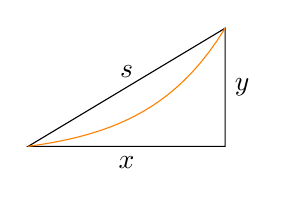
\begin{tikzpicture}[domain=0:2.5]
\draw (0,0) --node[below] {$\diff x$} (2.5,0) --node[right] {$\diff y$} (2.5,1.5) --node[left,above] {$\diff s$} cycle;
\draw[color=orange] plot (\x,{1.5/(exp(2.5)-1)*(exp(\x)-1)});
\end{tikzpicture}
\end{center}
\[\diff s=\sqrt{\diff x^2+\diff y^2}=\sqrt{1+\lrp{\dfrac{\diff y}{\diff x}}^2}\diff x\]
\begin{enumerate}
	\item 直角坐标
	\[\diff s^2=(1+[f'(x)]^2)\diff x^2\]
	\item 参数方程
	\[\diff s^2=([x'(t)]^2+[y'(t)]^2)\diff t^2\]
	\item 极坐标(通过$x=r(\theta)\cos\theta,y=r(\theta)\sin\theta$转直角坐标推导)
	\[\diff s^2=r^2\diff\theta^2+\diff r^2\]
\end{enumerate}

\subsection{面积}
\subsubsection{平面曲线}
\begin{enumerate}
	\item 直角坐标
	\[\diff A=y\diff x=(f(x)-g(x))\diff x\]
	积分上下限即两曲线端点
	\item 参数方程$(x(t),y(t)),t\in[\alpha,\beta]$(简单闭曲线$\Gamma$,端点相连$x(\alpha)=x(\beta),y(\alpha)=y(\beta)$,其他地方不相交\footnote{规定曲线的正向:沿着曲线的正向走,其包围的有界区域始终在曲线左侧})
	\[\diff A=y(t)\diff x(t)\implies A=\textcolor{red}{-}\oint_\Gamma y\diff x=\oint_\Gamma x\diff y=\frac{1}{2}\oint_\Gamma x\diff y-y\diff x\]
	积分上下限为$\alpha,\beta$
	\item 极坐标(曲线$r(\theta)$与向径$\theta=\alpha,\theta=\beta$所围成的区域)
	\[\diff A=\dfrac{1}{2}r^2(\theta)\diff\theta\]
	积分上下限为$\alpha,\beta$
\end{enumerate}
\begin{example}
求$r=3\cos\theta$和$r=1+\cos\theta$所围公共部分的面积
\end{example}
\begin{analysis}
两条曲线如下图所示,黄色部分即为要求的面积.
\begin{figure}[H]
\centering
\includegraphics[width=0.35\linewidth]{fig/polar_example.pdf}
\end{figure}
\par 注意在实际解题过程中,并没有图画作为辅助,因此需要自己判断积分区间.
\par 首先求定义域.
\[r\geq 0 \implies \theta\in[-\dfrac{\pi}{2},\dfrac{\pi}{2}]\]
\par 其次求出两曲线交点.
\[r=1+\cos\theta=3\cos\theta\implies\theta=\pm\dfrac{\pi}{3}\]
\par 判断对称性.
由于$\cos\theta$为偶函数,故两曲线都关于极轴对称.
\par 考虑内外关系,对小极径所在曲线进行积分.
\[A=2\cdot\dfrac{1}{2}\lrp{\intabu{0}{\frac{\pi}{3}}{(1+\cos\theta)^2}{\theta}+\intabu{\frac{\pi}{3}}{\frac{\pi}{2}}{(3\cos\theta)^2}{\theta}}=\dfrac{5}{4}\pi\]
\end{analysis}
\par 如果是单一极坐标曲线求面积,则一般关注其最大最小极径以及其对称性.

\subsubsection{空间曲面}
\label{subsubsec:surface_area}
思路与求曲线弧长类似,采用\textbf{切平面}来做原曲面的近似.
故要求$xOy$平面上微元$\diff x\diff y$对应的切平面的面积.
\begin{figure}[H]
\centering
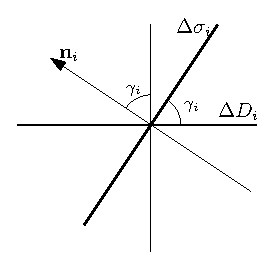
\includegraphics[width=0.2\linewidth]{fig/surface_projection.eps}
\end{figure}
\par 将曲面$z=f(x,y)$某点的切平面$\Delta\sigma$投影到平面$\Delta D$上,设$\diff S$的法向量$\vn=\pm(f_x,f_y,-1)$的方向余弦为$(\cos\alpha,\cos\beta,\cos\gamma)$,则
\[\diff S=\frac{\diff D}{|\cos\gamma|}=\frac{\diff x\diff y}{|\cos\gamma|}=\frac{\diff x\diff y}{1/\sqrt{f^2_x(x,y)+f^2_y(x,y)+1}}=\|\vn\|\diff x\diff y\]
\par 若曲面由参数形式给出
\[x=x(u,v),y=y(u,v),z=z(u,v),(u,v)\in D\]
\par 法向量采用叉积形式表示(见下图\footnote{图源:Parametric Representations of Surfaces, \url{https://services.math.duke.edu/education/ccp/materials/mvcalc/parasurfs/para3.html}}),则有
\[\diff S=\|\vr_u\diff u\times\vr_v\diff v\|=\|\vr_u\times\vr_v\|\diff u\diff v=|\vJ|\diff u\diff v\]
注意叉积的行列式即为平行四边形构成的面积,但要取绝对值.
实际上这里的叉积也即雅可比行列式(Jacobian)\footnote{准确来说是雅可比矩阵的行列式的绝对值,\url{http://faculty.bard.edu/belk/math352f11/Outline\%20-\%20Area.pdf}}.
\begin{figure}[H]
\centering
\includegraphics[width=0.4\linewidth]{fig/coordinate_projection2.png}
\end{figure}
记
\[\begin{aligned}
E&=|\mathbf{r}_u|^2=\lrp{\pd{x}{u}}^2+\lrp{\pd{y}{u}}^2+\lrp{\pd{z}{u}}^2\\
G&=|\mathbf{r}_v|^2=\lrp{\pd{x}{v}}^2+\lrp{\pd{y}{v}}^2+\lrp{\pd{z}{v}}^2\\
F&=\mathbf{r}_u\cdot\mathbf{r}_v=\pd{x}{u}\pd{x}{v}+\pd{y}{u}\pd{y}{v}+\pd{z}{u}\pd{z}{v}
\end{aligned}\]
进而曲面面积元
\[\diff S=\|\vr_u\times\vr_v\|\diff u\diff v=\sqrt{EG-F^2}\diff u\diff v\]
事实上,由这条式子也可以导出上面非参数方程的形式,考虑$\vr=(x,y,z(x,y))$,有
\[\vr_x\times\vr_y=\begin{bmatrix}\vi&\vj&\vk\\1&0&z_x\\0&1&z_y\end{bmatrix}=(-z_x,-z_y,1)\]


\begin{example}
求锥面$x^2+y^2=\dfrac{1}{3}z^2$与平面$x+y+z=2a(a>0)$所界部分的表面面积
\end{example}
\begin{analysis}
\begin{figure}[H]
\centering
\includegraphics[width=0.3\linewidth]{fig/surface_area_eg.pdf}
\end{figure}
锥面与平面的交线在$xOy$平面上的投影为(在下面这条曲线上不管取什么$z$值都成立,故为交线的投影)
\[3(x^2+y^2)=(2a-x-y)^2\implies x^2-xy+y^2+2a(x+y)=2a^2\]
由圆锥曲线理论\footnote{\url{https://math.stackexchange.com/questions/280937/finding-the-angle-of-rotation-of-an-ellipse-from-its-general-equation-and-the-ot}}知道旋转角
\[\theta=\frac{1}{2}\left|\arctan\frac{-1}{1-1}\right|=\pi/4\]
进而做转轴变换\footnote{\url{https://en.wikipedia.org/wiki/Rotation_(mathematics)}}
\[\begin{pmatrix}x\\y\end{pmatrix}=\begin{pmatrix}\cos\theta&-\sin\theta\\\sin\theta&\cos\theta\end{pmatrix}\begin{pmatrix}x'\\y'\end{pmatrix}\implies\begin{cases}x=\frac{x'+y'}{\sqrt{2}}\\y=\frac{-x'+y'}{\sqrt{2}}\end{cases}\]
得到射影方程为
\[\frac{(x'+2\sqrt{2})^2}{12a^2}+\frac{y'^2}{4a^2}=1\]
这是以$2\sqrt{3}a$和$2a$为半轴长的椭圆,面积为$\pi(2\sqrt{3}a)(2a)=4\sqrt{3}\pi a^2$.
锥面与平面所截部分的表面由截面$z=2a-x-y$和截出的锥面$z=\sqrt{3(x^2+y^2)}$两部分组成,因此
\[\begin{aligned}
S&=\iint_{D}\sqrt{1+(-1)^2+(-1)^2}\diff x\diff y+\iint_D\sqrt{1+\lrp{\frac{6x}{2\sqrt{3(x^2+y^2)}}}^2+\lrp{\frac{6y}{2\sqrt{3(x^2+y^2)}}}^2}\diff x\diff y\\
&=\iint_D(2+\sqrt{3})\diff x\diff y\\
&=(2+\sqrt{3})|D|=4(3+2\sqrt{3})\pi a^2
\end{aligned}\]
\end{analysis}

\subsection{体积}
\begin{enumerate}
	\item 旋转体(不是绕$x$轴、$y$轴旋转,则先做一个平移)
\[\diff V=\pi[f(x)]^2\diff x\]
	\item 已知截面积
\[\diff V=A(x)\diff x\]
\end{enumerate}

\subsection{曲率}
\begin{definition}[曲率]
用切线夹角与弧长之比来衡量曲线的弯曲程度,即
\[K=\left|\dfrac{\diff\varphi}{\diff s}\right|\]
\end{definition}
\begin{enumerate}
	\item 直角坐标
	\[K=\dfrac{|y''|}{(1+y'^2)^\frac{3}{2}}\]
	\item 参数方程(由参方推其他两个)
	\[K=\dfrac{|y''x'-y'x''|}{(x'^2+y'^2)^\frac{3}{2}}\]
	\item 极坐标
	\[K=\dfrac{|r^2+2r'^2-rr''|}{(r^2+r'^2)^\frac{3}{2}}\]
\end{enumerate}

\subsection{表面积}
旋转体的表面积可以通过以下的微元公式得到
\[\diff S=2\pi y\diff s\]
\par 注意想清楚取多少部分进行旋转,如上式的$y$仅仅是坐标轴一侧的$y$.
\begin{example}
求椭圆$\dfrac{x^2}{a^2}+\dfrac{y^2}{b^2}=1$绕$x$轴旋转所得旋转体的表面积
\end{example}
% http://www.nabla.hr/CL-DefiniteIntAppl5.htm
\begin{analysis}
本题解题方法来源于\footnote{Math StackExchange - How to Find the Surface Area of Revolution of An Ellipsoid from Ellipse Rotating, \url{https://math.stackexchange.com/questions/1379341}}.
对椭圆隐函数求导得
\[\frac{2x\diff x}{a^2} + \frac{2y\diff y}{b^2} = 0\]
故
\[\diff s = \sqrt{1 + (\frac{\diff y}{\diff x})^2}\diff x = \frac{1}{a^2}\,\frac{\diff x}{y}\,\sqrt{b^4x^2 + a^4y^2}\]
进而
\[\diff S = 2\pi y\diff s=2\pi \frac{1}{a^2}\,\sqrt{b^4x^2 + a^4y^2}\diff x\]
两边进行积分有
\[S = 2\frac{2\pi}{a^2}\int_{0}^{a} \sqrt{b^4x^2 + a^4y^2}\diff x\]
将
\[y^2 = b^2 - \frac{b^2}{a^2}\,x^2\]
代入有
\[S = 4\pi\,\frac{b}{a}\int_{0}^{a} \sqrt{a^2 - \varepsilon^2x^2}\diff x\]
其中,$\varepsilon^2=\sqrt{a^2-b^2}\Big/a^2$为椭圆离心率的平方,参数方程$x=a\sin\theta$
\[S = 4\pi\,ab\,\int_{0}^{\frac{\pi}{2}} \sqrt{1 - \varepsilon^2\sin^2\theta}\,\cos\theta\diff\theta\]
三角代换,令$\sin\phi = \varepsilon\sin\theta$,则$\cos\phi\diff\phi = \varepsilon\cos\theta\diff\theta$,故
\[S = 4\pi\,\frac{ab}{\varepsilon}\,\int\cos^2\phi\diff\phi\]
直接对其积分即可,将结果逐步回代得
\[S = 
2\pi\,\frac{ab}{\varepsilon}\lrp{\arcsin(\varepsilon) + \varepsilon\,\frac{b}{a}}= 
2\pi\,b^2\lrp{1 + \frac{a}{b}\,\frac{\arcsin(\varepsilon)}{\varepsilon}}\]
\end{analysis}

\subsection{物理量}
\subsubsection{质心}
平面的情况
\begin{theorem}[古鲁金(Guldin)第一定理]
质量分布均匀的平面曲线弧的质心坐标$(\bar{x},\bar{y})$由下式得出
\[2\pi\bar{x}l=S_1\qquad 2\pi\bar{y}l=S_2\]
其中,$S_1$和$S_2$分别为曲线弧绕$y$轴和绕$x$轴所得旋转体的侧面积,$l$为弧长.
\end{theorem}
其基本思想即将旋转体的侧面积转化为圆柱的侧面积.
\begin{theorem}[古鲁金第二定理]
质量分布均匀的平面图形绕此平面上一条与之不相交的直线旋转,所得旋转体的体积由下式给出
\[V=2\pi\bar{y}S\]
\end{theorem}
空间的情况
\[\bar{x}=\frac{\int_\Omega x\rho(P)\diff\Omega}{\int_\Omega\rho(P)\diff\Omega}=\frac{\int_\Omega x\diff m}{\int_\Omega\diff m}\]

\subsubsection{转动惯量}
\[\begin{aligned}
I_x&=\iiint_V(y^2+z^2)\rho(x,y,z)\diff x\diff y\diff z\\
I_{xy}&=\iiint_Vz^2\rho(x,y,z)\diff x\diff y\diff z
\end{aligned}\]

\subsubsection{引力}
\[\begin{aligned}
F_x&=\iiint_Vk\frac{x-x_0}{r^3}\rho(x,y,z)\diff x\diff y\diff z\\
\mathbf{F}&=F_x\vi+F_y\vj+F_z\vk
\end{aligned}\]